\documentclass[12pt]{article}
\usepackage{amsmath}
\usepackage{geometry}
\usepackage{tikz}
\usepackage{siunitx}

\geometry{a4paper, margin=1in}

\title{New Practice Problems in Magnetism}
\author{}
\date{\today}

\begin{document}

\maketitle

\section*{New Practice Problems}

\subsection*{Problem 1: Alpha Particle in a Magnetic Field}

\subsubsection*{Question}
An alpha particle ($q = +2e, m = 6.64 \times 10^{-27}$ kg) is accelerated from rest through a potential difference of \SI{2.0}{\kilo\volt}. It then enters a square region of uniform magnetic field $\vec{B}$ of magnitude \SI{0.15}{\tesla}, directed into the page. The length of the square region is $L=\SI{5}{cm}$. The particle enters at the middle of the left edge, moving horizontally.
\begin{enumerate}
    \item What is the speed of the alpha particle as it enters the magnetic field?
    \item Calculate the radius of its circular path inside the field.
    \item Determine the coordinates $(x, y)$ where the particle exits the field, assuming the entrance point is $(0, 0)$.
\end{enumerate}

\begin{center}
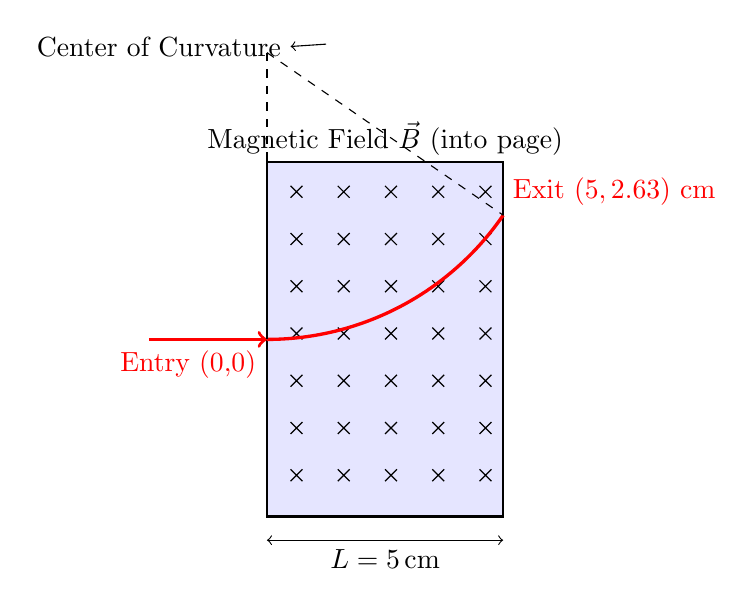
\begin{tikzpicture}[scale=1.5]
    % Draw the magnetic field region
    \fill[blue!10] (0, -1.5) rectangle (2, 1.5);
    \draw[thick] (0, -1.5) -- (0, 1.5) -- (2, 1.5) -- (2, -1.5) -- cycle;
    \node at (1, 1.7) {Magnetic Field $\vec{B}$ (into page)};
    % Draw B-field crosses
    \foreach \x in {0.2, 0.6, 1.0, 1.4, 1.8}
        \foreach \y in {-1.2, -0.8, -0.4, 0, 0.4, 0.8, 1.2}
            \draw (\x, \y) -- ++(0.1, 0.1) (\x, \y) ++ (0.1, 0) -- ++(-0.1, 0.1);
    
    % Draw the particle path
    \draw[->, red, very thick] (-1, 0) -- (0,0) node[below left] {Entry (0,0)};
    \draw[red, very thick] (0,0) arc (270:270+55.46:2.428); % r=6.07cm, scale=1.5->2.428
    
    % Annotations
    \coordinate (C) at (0, 2.428); % Center of circle
    \draw[dashed] (C) -- (0,0);
    \draw[dashed] (C) -- (2, 1.052); % Exit point
    \node[red, above right] at (2, 1.052) {Exit $(5, 2.63)$ cm};
    \draw[<->] (0, -1.7) -- (2, -1.7) node[midway, below] {$L = \SI{5}{cm}$};
    \draw[->] (0.5, 2.5) -- (0.2, 2.48) node[left] {Center of Curvature};
\end{tikzpicture}
\end{center}


\subsubsection*{Explanation}
This problem combines energy conservation, the magnetic force on a moving charge, and circular motion kinematics.
\begin{enumerate}
    \item First, we find the kinetic energy gained from the electric potential and use it to calculate the particle's speed.
    \item Next, we use the formula for the radius of circular motion in a B-field, $r = \frac{mv}{qB}$.
    \item Finally, we use geometry to find the exit point. We construct a right-angled triangle involving the center of the circle, the entry point, and the exit point to find the vertical displacement.
\end{enumerate}


\subsubsection*{Solution}
\begin{enumerate}
    \item \textbf{Speed of the particle:}
    The kinetic energy gained is equal to the change in electric potential energy:
    $$ KE = qV $$
    $$ \frac{1}{2}mv^2 = qV \implies v = \sqrt{\frac{2qV}{m}} $$
    \begin{align*}
        v &= \sqrt{\frac{2(2 \times 1.6 \times 10^{-19} \, \text{C})(\SI{2000}{\volt})}{6.64 \times 10^{-27} \, \text{kg}}} \\
          &= \SI{4.39e5}{\meter\per\second}
    \end{align*}

    \item \textbf{Radius of path:}
    \begin{align*}
       r &= \frac{mv}{qB} = \frac{(6.64 \times 10^{-27} \, \text{kg})(\SI{4.39e5}{\meter\per\second})}{(2 \times 1.6 \times 10^{-19} \, \text{C})(\SI{0.15}{\tesla})} \\
         &= \SI{0.0607}{\meter} \quad \text{or} \quad \SI{6.07}{\centi\meter}
    \end{align*}

    \item \textbf{Exit coordinates:}
    The particle travels a horizontal distance $L = \SI{5}{cm}$. We find the angle of deflection $\theta$ from the center of the circular path.
    $$ \sin\theta = \frac{L}{r} = \frac{\SI{5.0}{cm}}{\SI{6.07}{cm}} = 0.8237 $$
    $$ \theta = \arcsin(0.8237) = 55.46^\circ $$
    The vertical displacement $y$ is given by:
    $$ y = r - r\cos\theta = r(1-\cos\theta) $$
    $$ y = (\SI{6.07}{cm})(1 - \cos(55.46^\circ)) = (\SI{6.07}{cm})(1 - 0.567) = \SI{2.63}{cm} $$
    Since the force is initially upwards (Right-Hand Rule), the exit coordinates are $(x, y) = (\SI{5.0}{cm}, \SI{2.63}{cm})$.
\end{enumerate}


\newpage
\subsection*{Problem 4: Mass Spectrometer}

\subsubsection*{Question}
A sample containing two singly ionized isotopes of magnesium, ${}^{24}\text{Mg}^{+}$ ($m = 23.985$ amu) and ${}^{26}\text{Mg}^{+}$ ($m = 25.983$ amu), is analyzed in a mass spectrometer. The ions are first accelerated from rest by a potential difference of 500 V. They then enter a velocity filter consisting of a uniform electric field $E = 2.0 \times 10^4$ V/m and a uniform magnetic field $B_1$. Only ions of a specific velocity pass through undeflected. These selected ions then enter a second region with only a magnetic field $B_2 = 0.25$ T, perpendicular to their velocity. Calculate the separation distance between the landing spots of the two isotopes on the detector.
($1 \text{ amu} = 1.66 \times 10^{-27}$ kg)

\begin{center}
% CORRECTED DIAGRAM
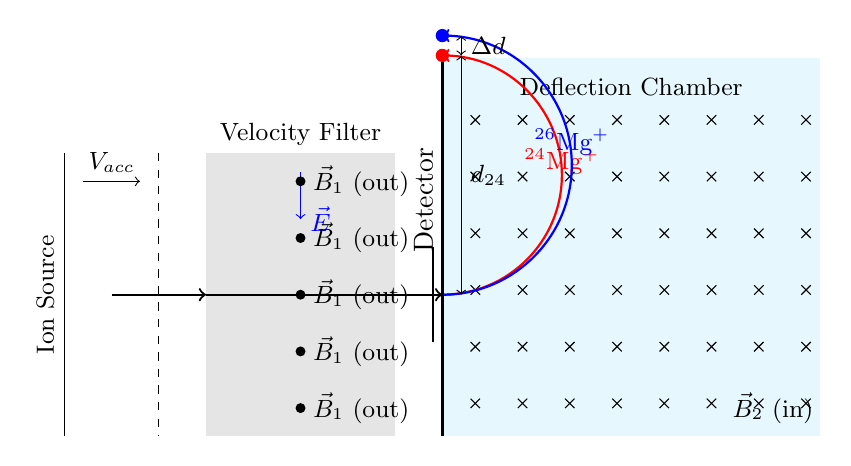
\begin{tikzpicture}[scale=1.2, font=\small]
    % Ion Source and Accelerator
    \draw (0,1.5) -- (0,-1.5);
    \draw[dashed] (1,1.5) -- (1,-1.5);
    \draw[->] (0.2, 1.2) -- (0.8, 1.2); \node at (0.5, 1.4) {$V_{acc}$};
    \node[rotate=90] at (-0.2, 0) {Ion Source};
    \draw[->, thick] (0.5, 0) -- (1.5, 0);

    % Velocity Filter
    \fill[gray!20] (1.5, -1.5) rectangle (3.5, 1.5);
    \node at (2.5, 1.7) {Velocity Filter};
    \draw[->, blue] (2.5, 1.3) -- (2.5, 0.8) node[right] {$\vec{E}$};
    \foreach \y in {-1.2, -0.6, 0, 0.6, 1.2}
        \fill (2.5, \y) circle (1.5pt) node[right=1pt] {$\vec{B}_1$ (out)};
    \draw[->, thick] (1.5, 0) -- (4, 0);
    \draw[thick] (3.9,-0.5) -- (3.9,0.5); % Slit
    \draw[thick] (4.1,-0.5) -- (4.1,0.5);

    % Deflection Chamber
    \fill[cyan!10] (4, -1.5) rectangle (8, 2.5);
    \node at (6, 2.2) {Deflection Chamber};
    % B2 field into page (correct for upward force)
    \foreach \x in {4.3, 4.8, 5.3, 5.8, 6.3, 6.8, 7.3, 7.8}
        \foreach \y in {-1.2, -0.6, 0, 0.6, 1.2, 1.8}
            \draw (\x, \y) -- ++(0.1, 0.1) (\x, \y) ++ (0.1, 0) -- ++(-0.1, 0.1) node[above right=1pt, color=cyan!50!black] {};
    \node at (7.5, -1.2) {$\vec{B}_2$ (in)};

    % Paths (Corrected to curve UP and land on the vertical detector)
    \def\rTwentyFour{1.266} % Scaled radius for Mg-24
    \def\rTwentySix{1.371}  % Scaled radius for Mg-26
    \draw[->, thick, red] (4, 0) arc (-90:90:\rTwentyFour); \node[red, above] at (4+\rTwentyFour, \rTwentyFour-0.1) {${}^{24}$Mg$^{+}$};
    \draw[->, thick, blue] (4, 0) arc (-90:90:\rTwentySix); \node[blue, above] at (4+\rTwentySix, \rTwentySix) {${}^{26}$Mg$^{+}$};

    % Detector
    \draw[very thick] (4, -1.5) -- (4, 2.5);
    \node[rotate=90, font=\normalsize] at (3.8, 1) {Detector};
    % Annotations for landing spots
    \coordinate (L24) at (4, 2*\rTwentyFour);
    \coordinate (L26) at (4, 2*\rTwentySix);
    \fill[red] (L24) circle (2pt);
    \fill[blue] (L26) circle (2pt);
    \draw[<->] (4.2, 0) -- (4.2, 2*\rTwentyFour) node[midway, right]{$d_{24}$};
    \draw[<->] (4.2, 2*\rTwentyFour) -- (4.2, 2*\rTwentySix) node[midway, right]{$\Delta d$};
\end{tikzpicture}
\end{center}


\subsubsection*{Explanation}
This problem involves three stages:
\begin{enumerate}
    \item \textbf{Acceleration:} Ions gain kinetic energy from a potential difference.
    \item \textbf{Velocity Filter:} Only ions with a specific velocity $v = E/B_1$ are selected.
    \item \textbf{Deflection:} In the second B-field, ions move in a semicircle. The radius depends on their mass, causing them to strike a vertical detector at different heights, $d=2r$, which leads to separation.
\end{enumerate}

\subsubsection*{Solution}
\begin{enumerate}
    \item \textbf{Find the speed of ${}^{24}\text{Mg}^{+}$ after acceleration:}
    $$ v_{24} = \sqrt{\frac{2qV}{m_{24}}} = \sqrt{\frac{2(1.6 \times 10^{-19})(500)}{23.985 \times 1.66 \times 10^{-27}}} = \SI{6.34e4}{\meter\per\second} $$
    We assume the velocity filter is tuned to this speed. Therefore, both isotopes that pass through must have this speed.

    \item \textbf{Path in the second magnetic field:}
    The ions travel in a semicircle of radius $r = \frac{mv}{qB_2}$. They strike the detector at a height of a diameter, $d = 2r$, from their entry point.
    $$ d = 2r = \frac{2mv}{qB_2} $$

    \item \textbf{Calculate landing positions:}
    For ${}^{24}\text{Mg}^{+}$:
    $$ d_{24} = \frac{2(23.985 \times 1.66 \times 10^{-27})(\SI{6.34e4}{\meter\per\second})}{(1.6 \times 10^{-19})(\SI{0.25}{\tesla})} = \SI{0.1266}{\meter} $$
    For ${}^{26}\text{Mg}^{+}$ (which also has speed $v=\SI{6.34e4}{\meter\per\second}$ to pass the filter):
    $$ d_{26} = \frac{2(25.983 \times 1.66 \times 10^{-27})(\SI{6.34e4}{\meter\per\second})}{(1.6 \times 10^{-19})(\SI{0.25}{\tesla})} = \SI{0.1371}{\meter} $$

    \item \textbf{Separation Distance:}
    The separation is the difference in the diameters of their paths.
    $$ \Delta d = d_{26} - d_{24} = 0.1371 - 0.1266 = \SI{0.0105}{\meter} = \SI{1.05}{\centi\meter} $$
\end{enumerate}

\end{document}